\chapter{Group Contract}
\label{app:groupcontract}


%% TEXT
\vspace*{1.0 cm}
\subsection*{Purpose}
The purpose of the contract is to achieve the best study environment and grades for the whole group.

\subsection*{§1. Compulsory Attendance}
Everyone will meet prepared on time. In case of illness or legitimate absence the group member must give notice in good time, so that changes to the meeting or project can be changed or postponed.

\subsection*{§2. Notification requirements}
Notices of change in working hours or place of work should be given to everyone in the group, so that it is possible to arrange time and place for the individual student.

\subsection*{§3. Democracy}
By disagreement or changes in a project the group will result the conflict by voting. In case of disagreement the group leader will have the deciding vote.

\subsection*{§4. Work Distribution}
The tasks shall be performed by members in approximately equal amounts. There are also opportunities to be assigned to tasks by the employees' abilities and desires, as long as this is feasible.

\subsection*{§5. Work Environment}
Project participants hereby undertake to contribute to a positive environment, where members must be treated with respect and value.

\subsection*{§6. Deadlines}
All deadlines will be held and task completed and delivered within the given time. In any unforeseen event, the student shall notice the group leader in good time.

\subsection*{§7. Breaches}
Any violation to the group contract will result with an oral and a written warning. With multiple breaches the student will be reported to the teacher for assessment of punishment.



\begin{figure}
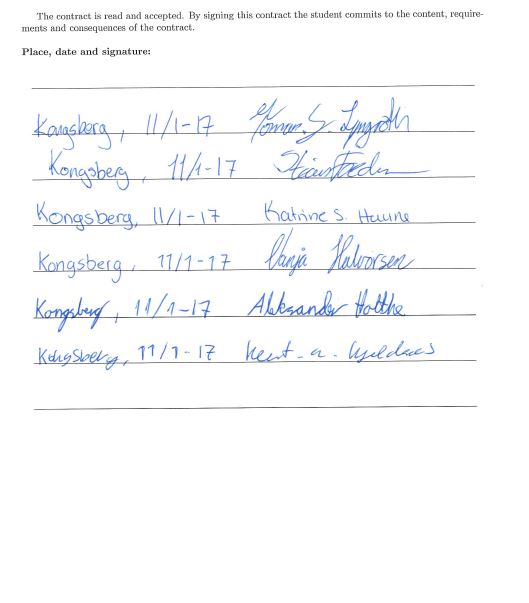
\includegraphics[scale = 1.6]{VAPIQ-PICTURES/gruppekontrakt.JPG}
\end{figure}





\begin{comment}
\vspace*{1 cm}
The contract is read and accepted. By signing this contract the student commits to the content, requirements and consequences of the contract.\\\\
\textbf{Place, date and signature:}\\

\begin{center}
\line(1,0){450}
\end{center}
\vspace*{0.5 cm}
\begin{center}
\line(1,0){450}
\end{center}
\vspace*{0.5 cm}
\begin{center}
\line(1,0){450}
\end{center}
\vspace*{0.5 cm}
\begin{center}
\line(1,0){450}
\end{center}
\vspace*{0.5 cm}
\begin{center}
\line(1,0){450}
\end{center}
\vspace*{0.5 cm}
\begin{center}
\line(1,0){450}
\end{center}
\vspace*{0.5 cm}
\begin{center}
\line(1,0){450}
\end{center}
\vspace*{0.5 cm}
\begin{center}
\line(1,0){450}
\end{center}

\end{comment}
